We were able to find traces of the files in Rick's computers.

We first started by looking at both the volumes partition information using the \textit{mmls} tool.

\begin{figure}[H]
    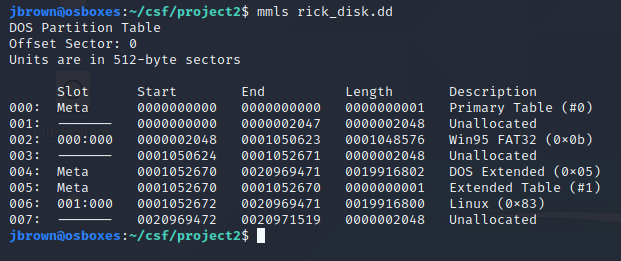
\includegraphics[scale=0.7]{mmls-rick}
    \centering
    \caption{Output of mmls rick\_disk.dd}
\end{figure}

\begin{figure}[H]
    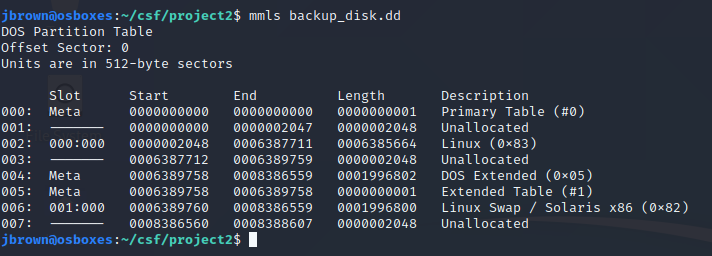
\includegraphics[scale=0.7]{mmls-backup}
    \centering
    \caption{Output of mmls backup\_disk.dd}
\end{figure}

From which we can conclude that are two filesystems in place in the first volume at the offsets 2048 and 1052672 and two filesystem in the second volume at offset 2048 and 6389760.

We started by analyzing the first volume at offset 1052672.

\begin{figure}[H]
    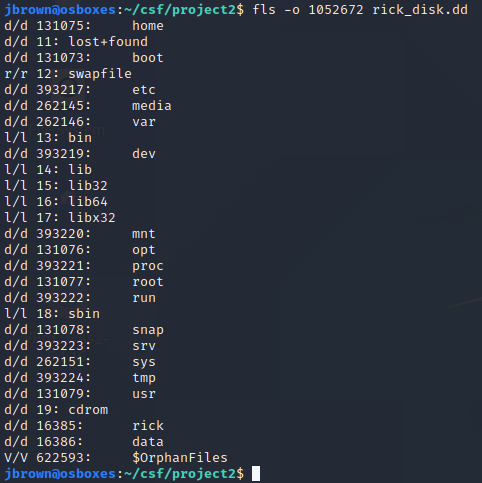
\includegraphics[scale=0.7]{fls-root-rick}
    \centering
    \caption{Output of fls -o 1052672 rick\_disk.dd}
\end{figure}

There is a directory named \textit{rick} which is not a default Linux directory so we decided to investigate it.

\begin{figure}[H]
    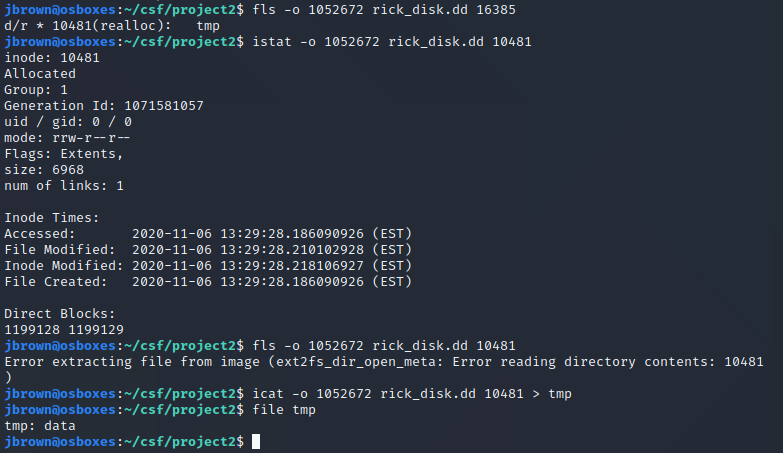
\includegraphics[scale=0.7]{search-rick-rick.png}
    \centering
    \caption{investigation of inode 16385 (/rick) in offset 1052672 rick\_disk.dd}
\end{figure}

Seems like there were some temporary files here that were deleted and can't be recovered so we abandoned this path and investigated the \textit{data} folder which is also not a default Linux directory.

\begin{figure}[H]
    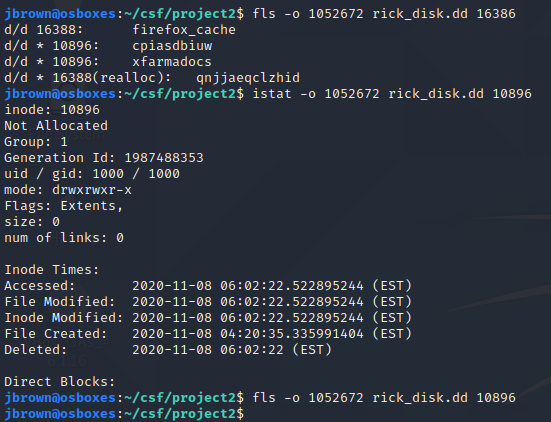
\includegraphics[scale=0.7]{search-data-rick.png}
    \centering
    \caption{investigation of inode 16386 (/data) in offset 1052672 rick\_disk.dd}
\end{figure}

There is some evidence here of the presence of the xFarma documents we are looking for.

The next directory to investigate was the \textit{/home/rick} directory. Here we found an \textit{assets} directory which we dove into.

\begin{figure}[H]
    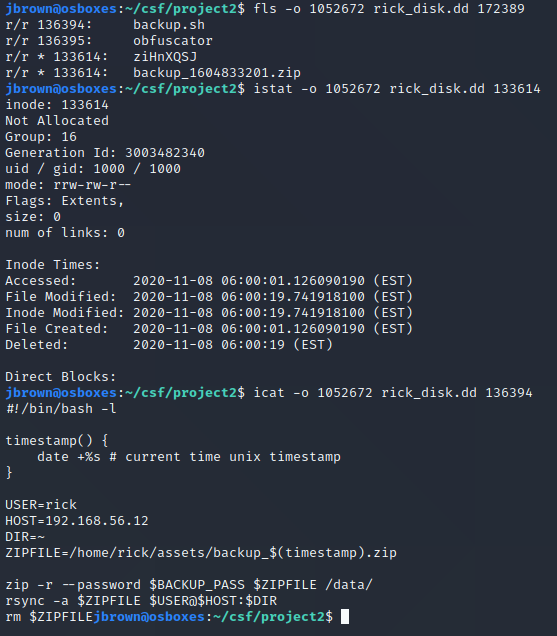
\includegraphics[scale=0.7]{search-home-assets-rick.png}
    \centering
    \caption{investigation of inode 172389 (/home/rick/assets) in offset 1052672 of rick\_disk.dd}
\end{figure}

Here we found a \textit{backup.sh} script which creates an encrypted .zip file of the \textit{/data} directory we found earlier with a password present in the \textit{BACKUP\_PASS} variable and then syncs this file with the remote backup server located on 192.168.56.12. We can also see that the local version was deleted in the meantime. Something important here is that this password is an environment variable available in the shell which means we should be able to find it if it hasn't been deleted.

We also looked at the \textit{.bash\_history} to see if there was something useful there.

\begin{figure}[H]
    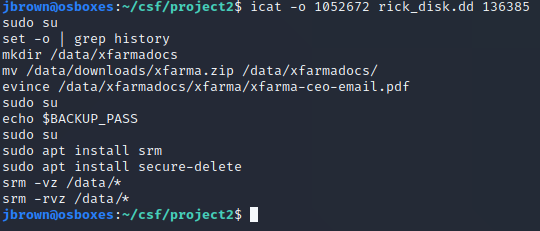
\includegraphics[scale=0.7]{search-home-bash_history-rick.png}
    \centering
    \caption{investigation of inode 136385 (/home/rick/.bash\_history) in offset 1052672 of rick\_disk.dd}
\end{figure}

Here we can again see evidence that the xFarma documents were present in this machine. We can also see that they have been deleted using a command line tool for secure deletion of files so we shouldn't be able to recover them. Maybe we can find them on the backup server.

Anyway let's keep looking for the \textit{BACKUP\_PASS} variable and try to find where it is defined. Most shell initialization variables are located on \textit{/etc/profile} so let's look it up.

\begin{figure}[H]
    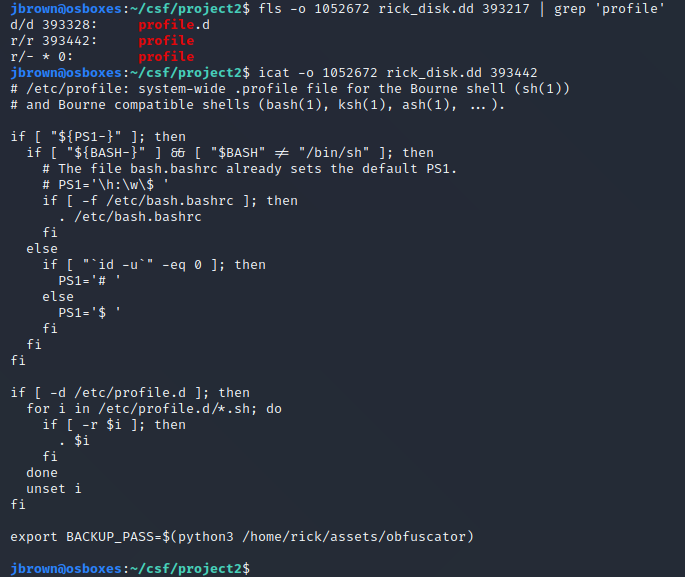
\includegraphics[scale=0.7]{search-etc-profile-rick.png}
    \centering
    \caption{investigation of inode 393442 (/etc/profile) in offset 1052672 of rick\_disk.dd}
\end{figure}

We found the \textit{BACKUP\_PASS} which seems to have as value the output of the python script located in \textit{/home/rick/assets/obfuscator}. If we run it we obtain the password \textit{\textbf{r1cK\_7ru7h2020\_CH1cK}}.

\begin{figure}[H]
    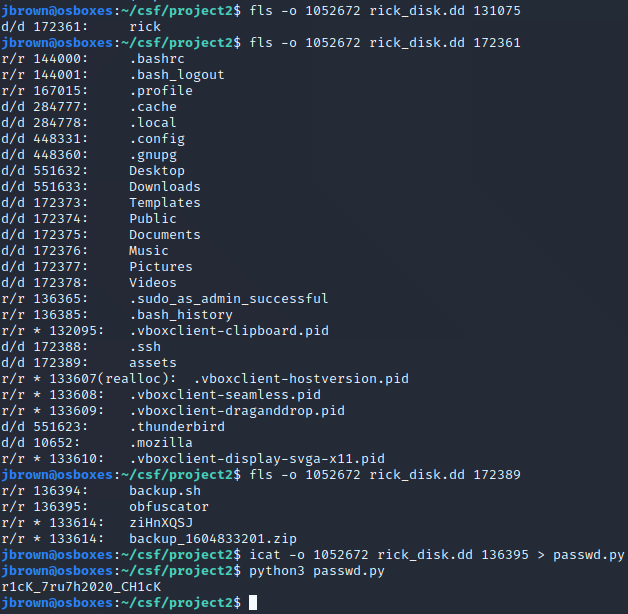
\includegraphics[scale=0.7]{search-home-assets-obfuscator-rick.png}
    \centering
    \caption{investigation of inode 136395 (/home/rick/assets/obfuscator) in offset 1052672 of rick\_disk.dd}
\end{figure}

Let's check the backup server now for the missing .zip file. From the \textit{backup.sh} script we learnt that the synced files are placed in the \textit{home} directory for the user rick.

\begin{figure}[H]
    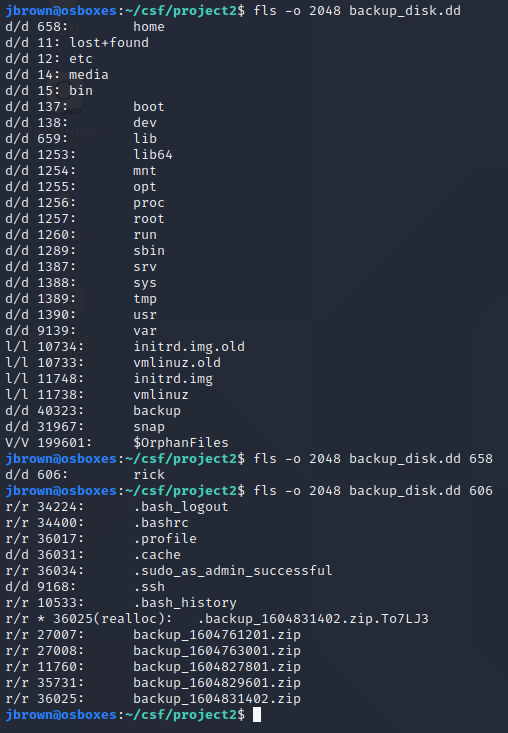
\includegraphics[scale=0.7]{fls-home-backup.png}
    \centering
    \caption{investigation of inode 606 (/home/rick/) in offset 2048 of backup\_disk.dd}
\end{figure}

The one we are looking for is the one with timestamp 1604833201, but it isn't here so let's use the latest one.

\begin{figure}[H]
    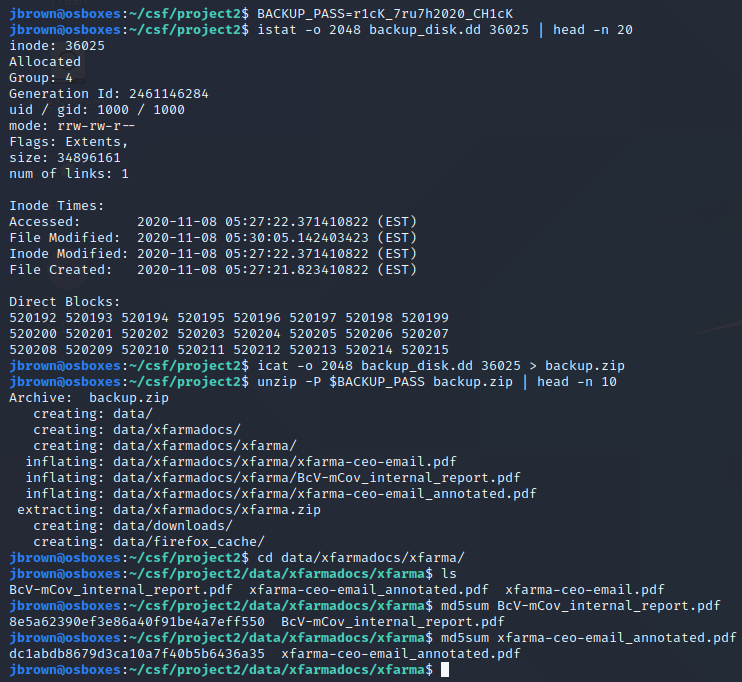
\includegraphics[scale=0.7]{search-home-backup-backup.png}
    \centering
    \caption{investigation of inode 36025 (/home/rick/) in offset 2048 of backup\_disk.dd}
\end{figure}

Here are the files we were looking for with the expected md5. This proves that the files were in Rick's computer. 